\section{Results}
\label{sec:results}

Beginning with the relative error in Figure \ref{fig:compare}, we see that the error in the mean energy has a decreasing trend all the way, while the error in absolute magnetisation seem to stabilise around a fixed value.
\begin{figure}[htbp]
	\centering
	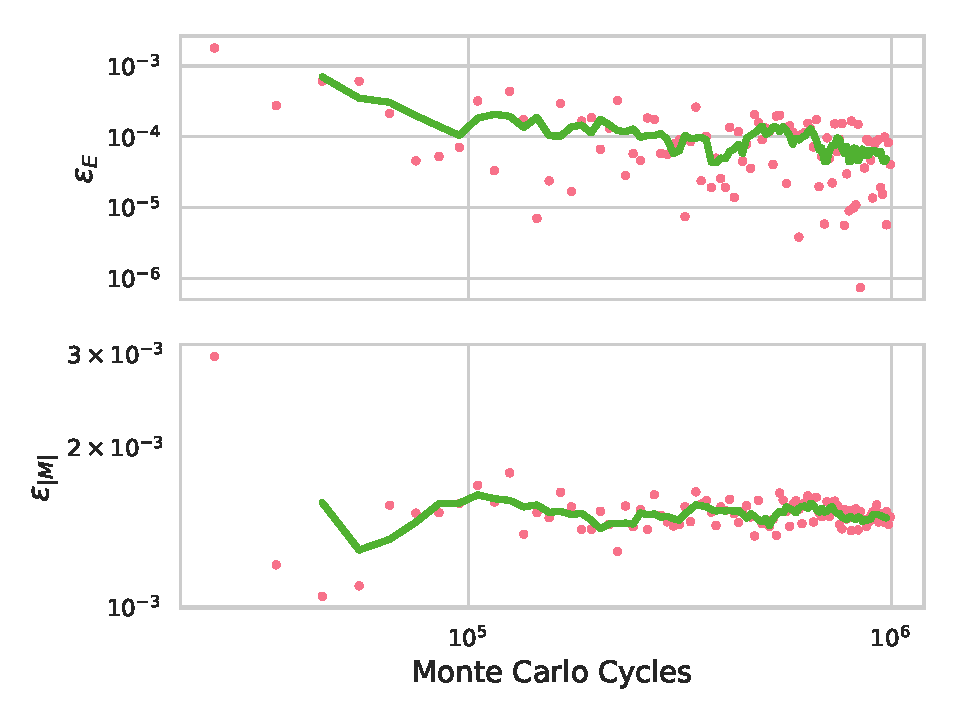
\includegraphics[width=0.5\textwidth]{relerror.pdf}
	\caption{Here we show the relative error of the mean energy and magnetisation as a function of Monte Carlo cycles in the case of a 2x2 lattice. We use the same random seed for each Monte Carlo cycle.}
	\label{fig:compare}
\end{figure}

In Figure \ref{fig:MC} we present the mean energy, and absolute magnetisation as functions of Monte Carlo cycles with both ordered and unordered initial states (see the Methods section for distinction). We see that both parameters converge rather rapidly for increasing Monte Carlo cycles, and in the $T=1.0$ case it happens almost immediately for the ordered lattice.
\begin{figure}[htbp]
	\centering
	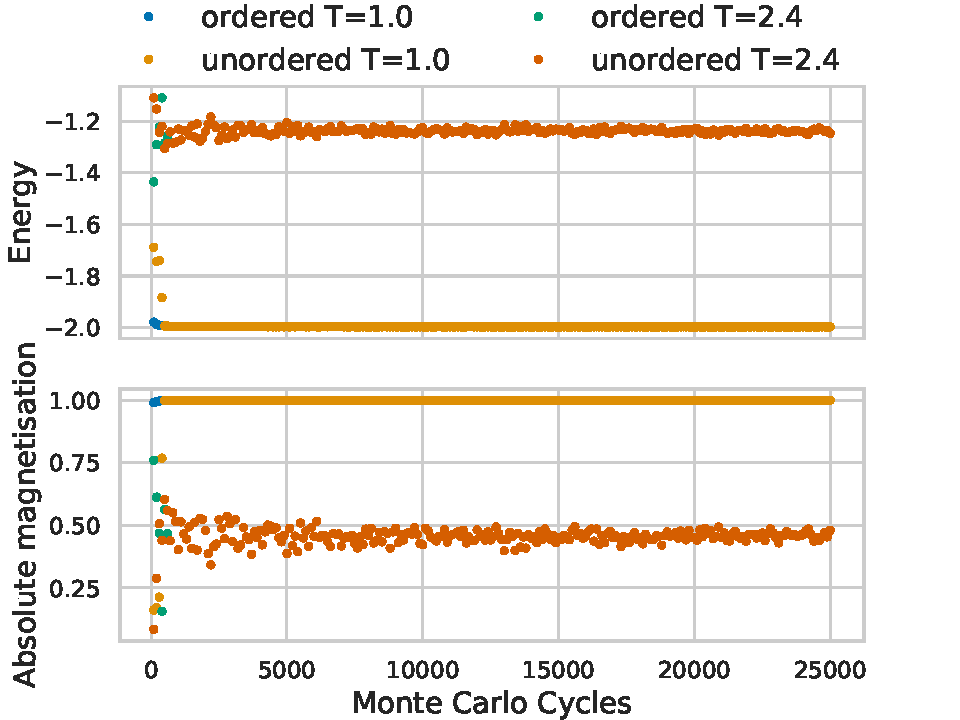
\includegraphics[width=0.5\textwidth]{MC.pdf}
	\caption{We compare between unordered and ordered initial lattices, i.e. a random lattice and a lattice where all elements are set to 1.}
	\label{fig:MC}
\end{figure}

Taking a closer look at the most likely state, we see the probability distribution of our Metropolis algorithm in Figure \ref{fig:probabilitydist}. For $T=1.0$ there looks to be few likely states, while for $T=2.4$ the distribution has a clearly defined interval of likely states between approximately $\expval{E} \in [-1.6, -0.8)$ with a peak at around $\expval{E} = -1.3$.
\begin{figure}[htbp]
	\centering
	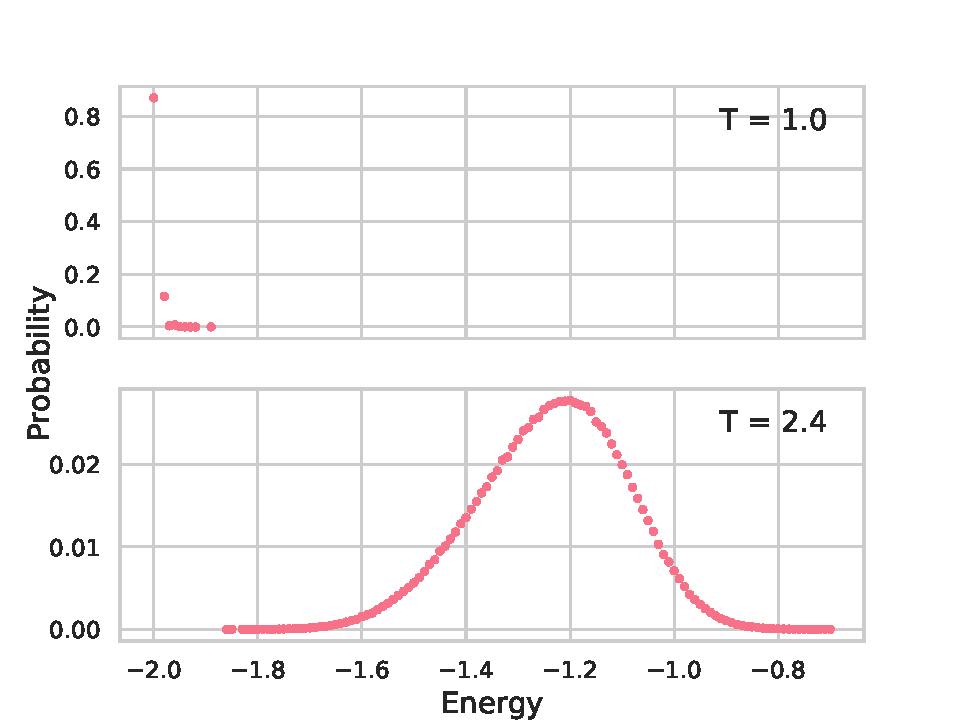
\includegraphics[width=0.5\textwidth]{probabilitydist.pdf}
	\caption{Shown here is the probability distribution obtained from the Metropolis algorithm for a $L=20$ lattice over $10^6$ Monte Carlo cycles.}
	\label{fig:probabilitydist}
\end{figure}

Shown in Figure \ref{fig:energy001} is the mean energy of the system. We see that there is a steady increase with little difference between lattice sizes.
\begin{figure}[htbp]
	\centering
	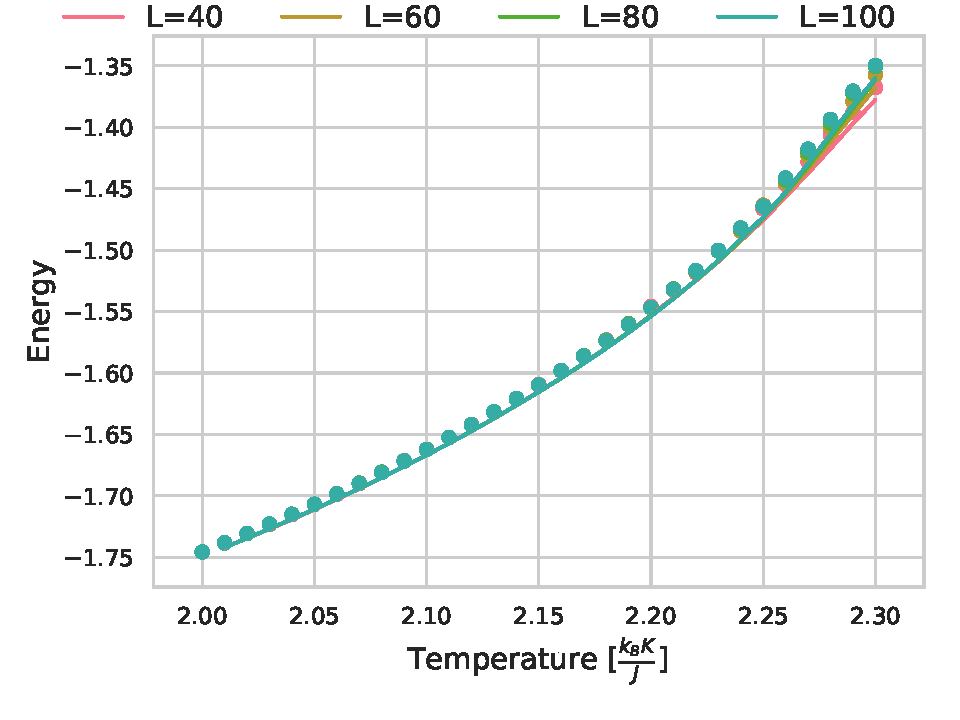
\includegraphics[width=0.5\textwidth]{Energy001.pdf}
	\caption{Mean energy as a function of $T \in[2.0, 2.3]$ for selected lattice sizes $L = 40, 60, 80, 100$.}
	\label{fig:energy001}
\end{figure}

Considering now the absolute magnetisation (see Figure \ref{fig:absmag}), we observe a steady decline with little distinction between lattices until around $T=2.25$, where the graphs slightly diverge with a lower minima for larger lattices.
\begin{figure}[htbp]
	\centering
	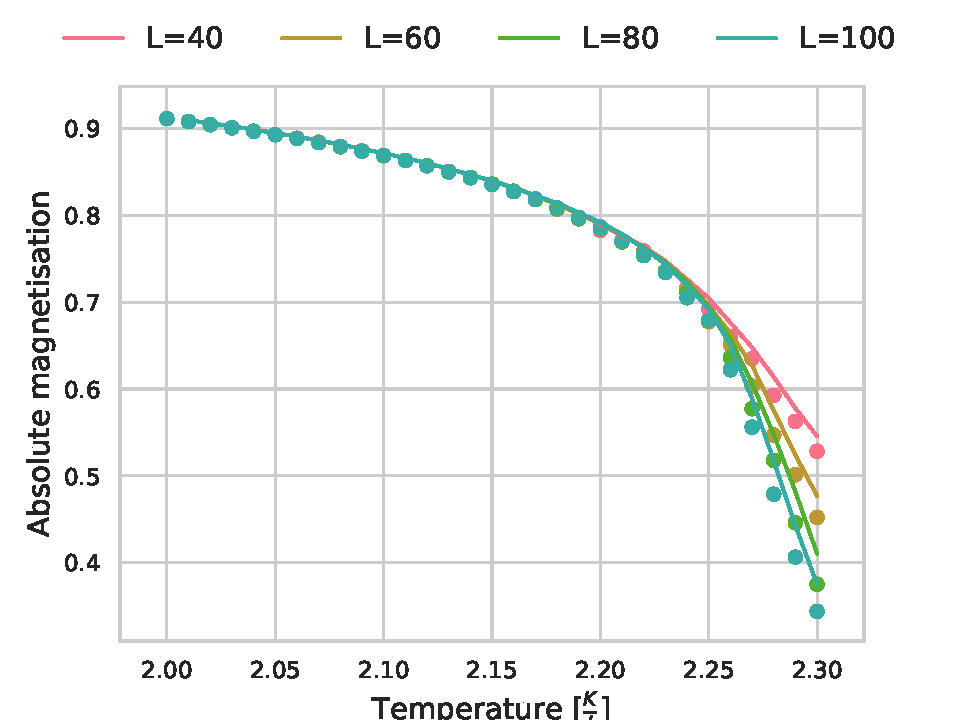
\includegraphics[width=0.5\textwidth]{Absolute_magnetisation001.pdf}
	\caption{Absolute magnetisation as a function of $T \in[2.0, 2.3]$, for selected lattice sizes $L = 40, 60, 80, 100$.}
	\label{fig:absmag}
\end{figure}

Looking now at the heat capacity in Figure \ref{fig:heatcap001} we see a steady increase for all lattices, akin to the mean energy, until around $T=2.2$. After $T=2.25$ we can clearly distinguish between lattices. We also observe higher maxima for larger lattices, and in the case of $L=60, 80, 100$, we observe a decrease after around $T=2.26$.
\begin{figure}[htbp]
	\centering
	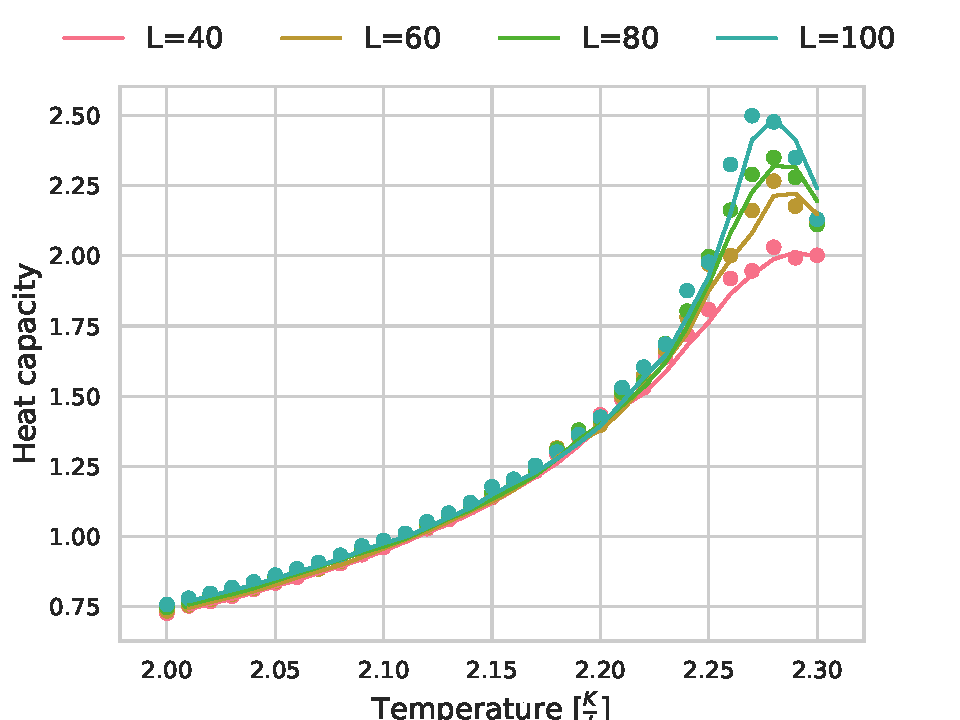
\includegraphics[width=0.5\textwidth]{Heat_capacity001.pdf}
	\caption{Specific heat capacity as a function of $T \in[2.0, 2.3]$, for selected lattice sizes $L = 40, 60, 80, 100$.}
	\label{fig:heatcap001}
\end{figure}

The susceptibility as a function of temperature is shown in Figure \ref{fig:susceptibility001}. There is little change until around $T=2.1$ when the susceptibility starts slowly increasing until around 2.25 where it increases quicker for $L=40, 60$ and rapidly for $L=80, 100$, attaining higher maxima for larger lattices.
\begin{figure}[htbp]
	\centering
	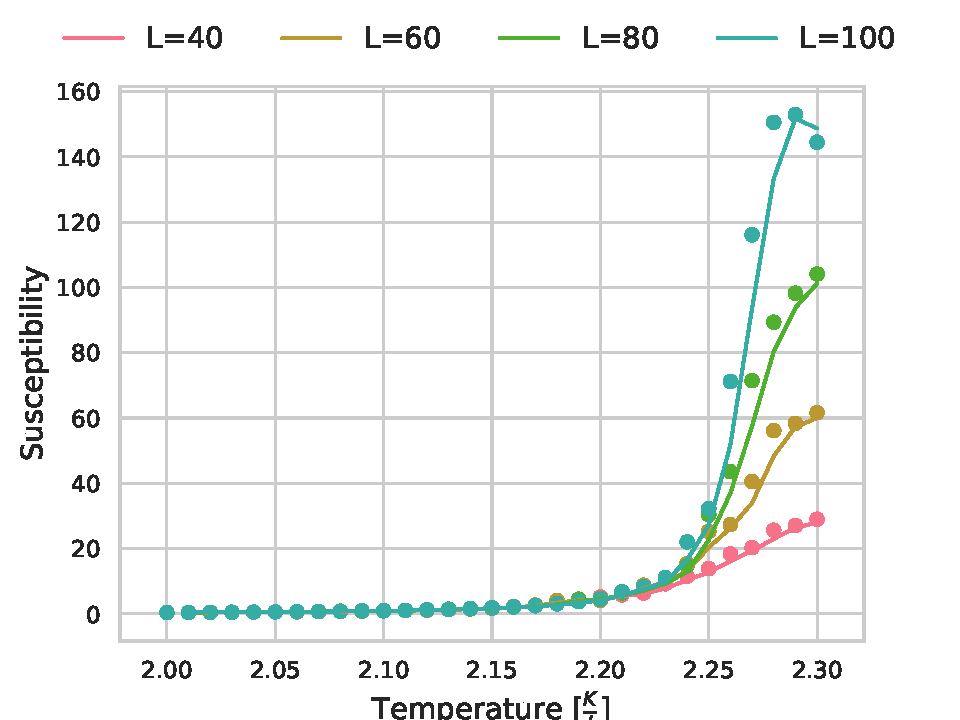
\includegraphics[width=0.5\textwidth]{Susceptibility001.pdf}
	\caption{Susceptibility as a function of $T \in[2.0, 2.3]$, for selected lattice sizes $L = 40, 60, 80, 100$.}
	\label{fig:susceptibility001}
\end{figure}

Zooming in on the heat capacity in the interval $T \in [2.26, 2.30]$ we get a closer look at the maximum's (see Figure \ref{fig:heatcap}). We find the temperature at the respective maxima numerically, which using eq. \ref{eq:criticalT} yielded the critical temperature, shown in Table \ref{table:Tmax}.
\begin{figure}[htbp]
	\centering
	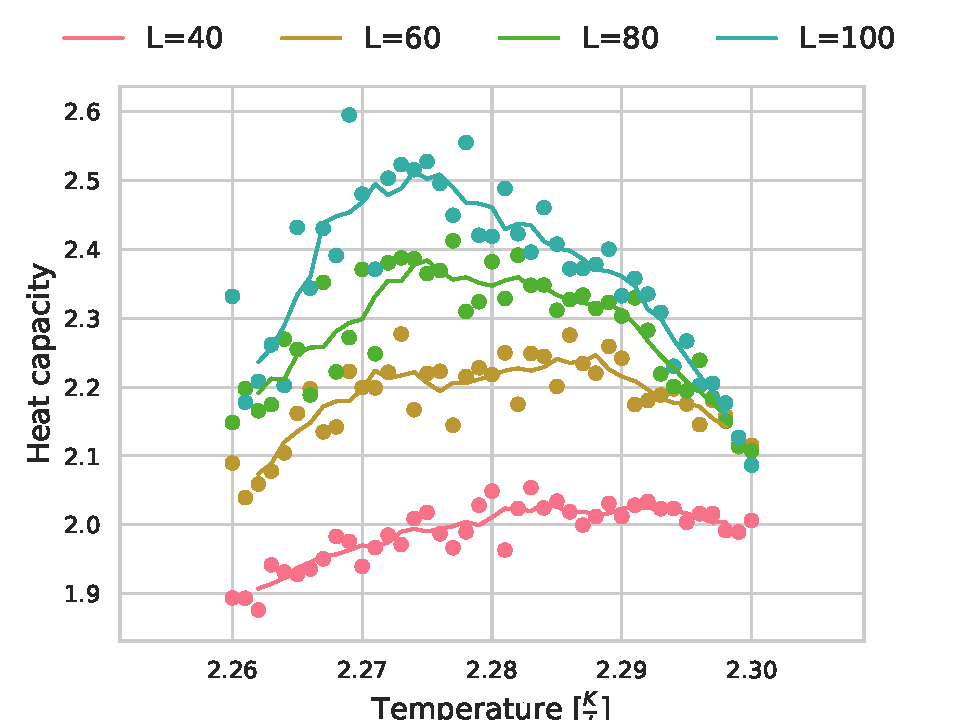
\includegraphics[width=0.5\textwidth]{Heat_capacity0001.pdf}
	\caption{Restricting the temperature domain to $[2.26, 2.30]$ we take a closer look at the heat capacity as a function of temperature for lattice sizes $L=40, 60, 80, 100$. Here the graph is obtained from a rolling mean with window 4}
	\label{fig:heatcap}
\end{figure}

\begin{table}[htbp]
	\centering
	\begin{tabular}{l|cccc}
		\textbf{$dT$} & $dT_0$ & $dT_0 \qty(RM)$ & $dT_1$ & $dT_1 \qty(RM)$  \\
		\midrule
		\addlinespace[0.1cm]

		\textbf{$T_C$} & 2.263 & 2.273 & 2.260 & 2.267 \\
	\end{tabular}
	\caption{Critical temperature for $dT_0 = 0.01$ and $dT_1 = 0.001$ with and without rolling mean, windows size 2 and 5 respectively.}
	\label{table:Tmax}
\end{table}

We produced more figures, which can be found in the appendix.
